\section{Experimental Results} 
\label{sec:results} 
 
In this section, we discuss the performance results of several experiments on
a multicore Intel Xeon workstation and a Blue Gene/P (both at Argonne). The
workstation has dual quad-core E5462 Xeon processors (8 cores total) running
at 2.8 GHz (1600 MHz FSB) with 32 KB L1 cache, 12 MB of L2 cache (6 MB shared
per core pair), and 2 GB of DDR2 FBDIMM RAM, running Linux kernel version
2.6.25 (x86-64). Each compute node of the Blue Gene/P is equipped with four
850 MHz IBM PowerPC 450 processors with a dual floating-point unit and 2 GB
total memory per node, private L1 (32 KB) and L2 (4 MB) caches, a shared L3
cache (8 MB), and running a proprietary lightweight operating system. We used
version 10.1 of the Intel and version 9.0 of the IBM XL C/C++ V9.0 compilers
on the Xeon and Blue Gene/P, respectively. Because of space considerations,
here we discuss a limited number of computational kernels; more performance
results for different computations are available at the Orio project
website~\cite{OrioURL}.

\subsection{Sequence of Linear Algebra Operations} 
\label{sec:axpy4-results}
 
In this experiment, we tuned the performance of the AXPY-4 operation (see
Figure~\ref{fig:orio-example}) on a single node of the Blue Gene/P machine
using the IBM xlc compiler.  We measured the performance for two scenarios:
using a single core per node and using all four cores. The results are shown
in Figures~\ref{fig:axpy4-bgp-seq} and~\ref{fig:axpy4-bgp-par},
respectively. The single-core scenario was compiled with the following options:
\texttt{-O3 -qstrict -qarch=450d -qtune=450 -qhot -qsmp=noauto};  the
multicore scenario differs in the use of \texttt{-qsmp=auto} for the non-Orio
versions. The parallel Orio version contains OpenMP parallelization
directives in the generated code, thus necessitating the use of the
\texttt{-qsmp=omp:noauto} compiler option. Included are performance numbers for four
code variants: a simple loop implementation without any library calls
(labeled ``Compiler-optimized''), two BLAS-based implementations that use
Goto BLAS~\cite{Goto:2006fk} and the ESSL~\cite{ESSL} libraries, and the
Orio-tuned version.

\begin{figure}%[b]
\begin{tabular}{c}
\begin{minipage}[t]{.47\textwidth}
\centering
\vspace{0.2in}
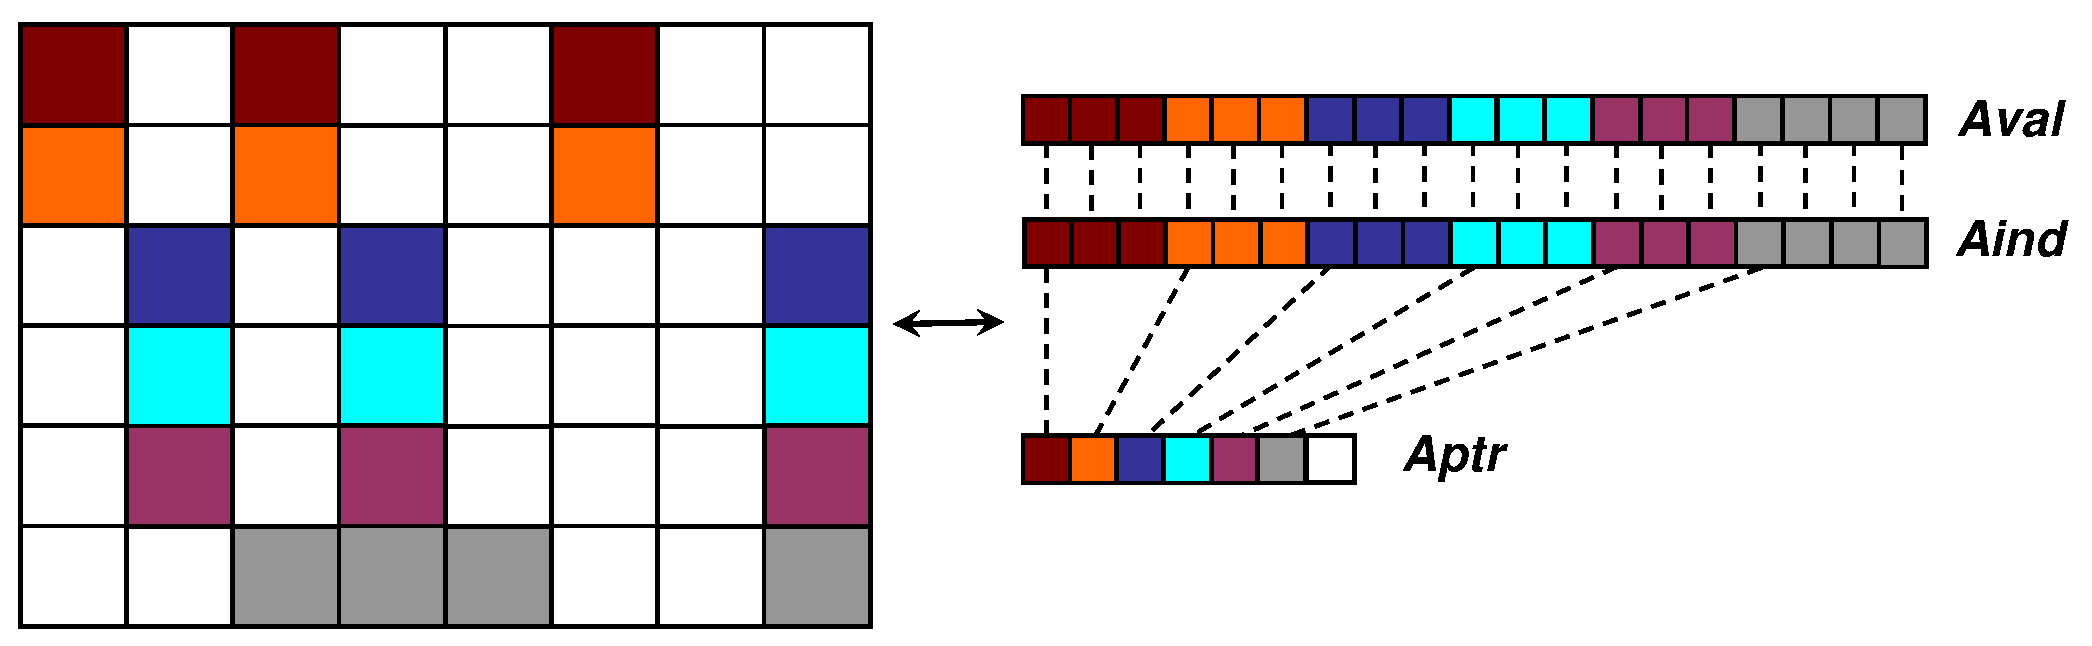
\includegraphics[width=1.0\textwidth]{figures/spmv.eps}  
\end{minipage}
\\
{\footnotesize (a)}
\\
\begin{minipage}[t]{.3\textwidth}
\scriptsize
\begin{verbatim}


for (i=0; i<num_rows; i++)
  for (j=Aptr[i]; j<Aptr[i+1]; j++)
    y[i] += Aval[j]*x[Aind[j]];

\end{verbatim}
\end{minipage}
\\
{\footnotesize (b)}
\\
\end{tabular}

\caption{(a) Compressed sparse row (CSR) format; (b) Basic implementation of CSR-based SpMV.}
\label{fig:spmv}
\end{figure}


\begin{figure*}%[t] 
\begin{center} 
  \subfigure[Sequential (single core)]{ 
  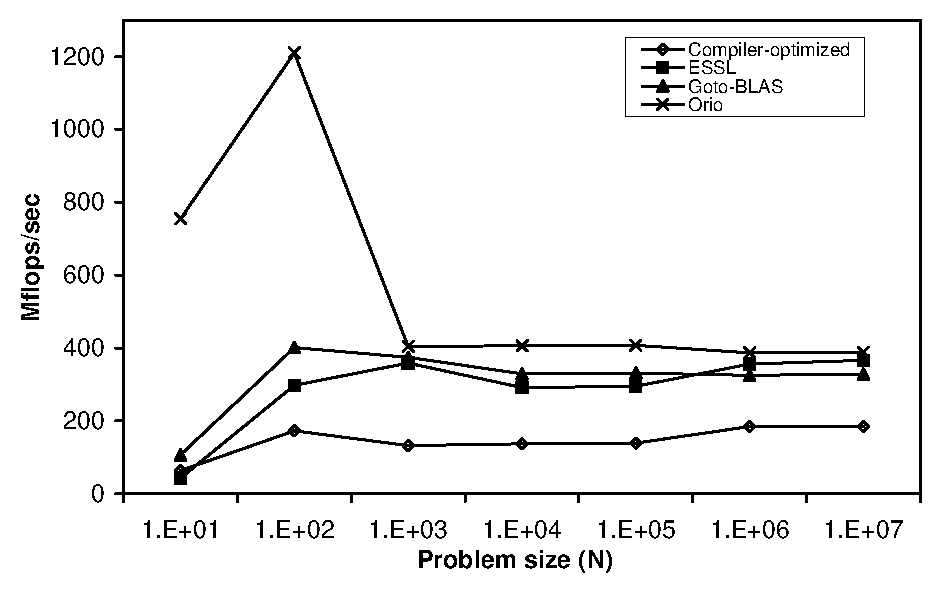
\includegraphics[width=.45\textwidth]{figures/axpy4_bgp/seq.eps}  
  \label{fig:axpy4-bgp-seq} 
  } 
  \subfigure[Parallel (four cores)]{ 
  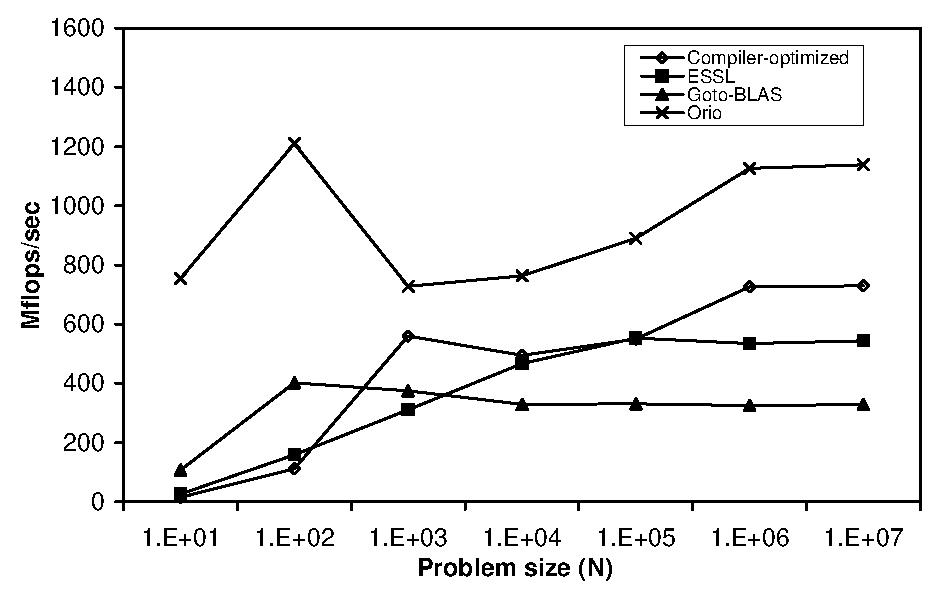
\includegraphics[width=.45\textwidth]{figures/axpy4_bgp/par.eps}  
  \label{fig:axpy4-bgp-par} 
  } 
\end{center}
\caption{Performance of AXPY-4 operations on the Blue Gene/P.} 
\label{fig:axpy4-bgp-results} 
\end{figure*} 




The performance results shown in Figure~\ref{fig:axpy4-bgp-results} indicate
that the code tuned by Orio consistently outperforms the other three versions
for both the sequential and parallel cases. We observe that even for a simple
algebraic operation, such as the composed AXPY routines, the compiler alone
is unable to yield performance comparable to the empirically tuned
version. Moreover, implementations that rely on calls to multiple tuned
library routines (e.g., Goto BLAS and ESSL) suffer from loss of both spatial
and temporal localities, resulting in inferior memory performance.
%The sequential BLAS-based implementation perform better than the
%sequential single loop implementation. while for the parallel case, the 
%simple loop implementation is more efficient than the BLAS codes.

\subsection{Sparse Matrix Computations} 

In this section we examine the effectiveness of Orio in optimizing key
computations in PETSc~\cite{petsc-user-ref}, a toolkit for the parallel
numerical solution of partial differential equations, by empirically tuning
one of its heavily used kernels, sparse matrix-vector multiplication
(SpMV). SpMV dominates the performance of various scientific applications;
yet, traditional implementations of sparse kernels exhibit relatively poor
performance because of the use of indirect addressing for accessing the
matrix data elements.
%In
%order to attain higher performance, SpMV requires selecting a compact data
%structure and code transformations that best exploit properties of both the
%sparse matrix and the underlying architecture. Hence, the need for
%optimization and runtime tuning is a big distinction from the dense
%matrix-vector multiplication.

The SpMV operation computes $\forall_{A_{i,j}} \neq 0:y_{i}
\leftarrow y_{i} + A_{i,j} \cdot x_{j}$, where $A$ is a sparse matrix,
and $x$, $y$ are dense vectors. Each element of $A$ is used precisely once,
and element reuse is possible only for $x$ and $y$. Thus, to optimize SpMV,
one should use compact data structures for $A$ and try to maximize temporal
reuse of $x$ and $y$. One of the most commonly used data structures for
storing a sparse matrix is compressed sparse row (CSR) storage
~\cite{vuduc-thesis},
illustrated in Figure~\ref{fig:spmv}(a). Elements in each row of $A$ are
packed together in a dense array, \texttt{Aval}, and a corresponding array of
integers \texttt{Aind} stores the column indices. The \texttt{Aptr} array
designates where each sparse row begins in \texttt{Aval} and
\texttt{Aind}. An implementation of SpMV using CSR storage is
shown in Figure~\ref{fig:spmv}(b).

PETSc's implementation of SpMV used in this experiment exploits matrix
structure by using \textit{inodes}, which represent rows with identical
nonzero structure.  PETSc detects inodes automatically in arbitrary sparse
matrices. For example, the sparse matrix shown in Figure~\ref{fig:spmv}(a)
contains three inodes. The first inode is of size two because it holds two
adjacent rows (i.e., the first and the second rows) with the same nonzero
structure. The second inode contains three consecutive rows with identical
nonzero structure, and the last inode has only a single row. Knowing the
properties of each inode at runtime enables maximum reuse of vector $x$ since
multiple elements of $x$ can be loaded and used exactly once for all rows in
the same inode structure. To accomplish this, one must use a
register-blocking transformation. To optimize the inode-based SpMV routine,
we incorporated a new transformation module inside Orio that implements
various optimization strategies including register blocking, SIMDization,
memory alignment optimization, loop-control optimization, accumulator
expansion, and thread-level parallelization (with OpenMP). We then used Orio
to automatically select the best version of the optimized inode SpMV. Only
the outer loop that iterates over inodes was parallelized by using OpenMP.

To evaluate the performance of the tuned SpMV routine, we conducted the
experiment using a 2-D driven cavity flow simulation
application~\cite{coff:kell:keye} (SNES ex27 in PETSc), on both the Xeon and
Blue Gene/P. The ``Compiler-optimized'' label is used as a base case that
represents the performance of the naive implementation of SpMV (shown in
Figure~\ref{fig:spmv}(b)) optimized by the native compiler. We also tested
the performance of the hand-tuned (by PETSc developers) SpMV code, which is
included in PETSc releases.



\begin{figure*}%[ht]
\begin{center} 
  \subfigure[SMP: $p=1$, $t/p=8$]{
  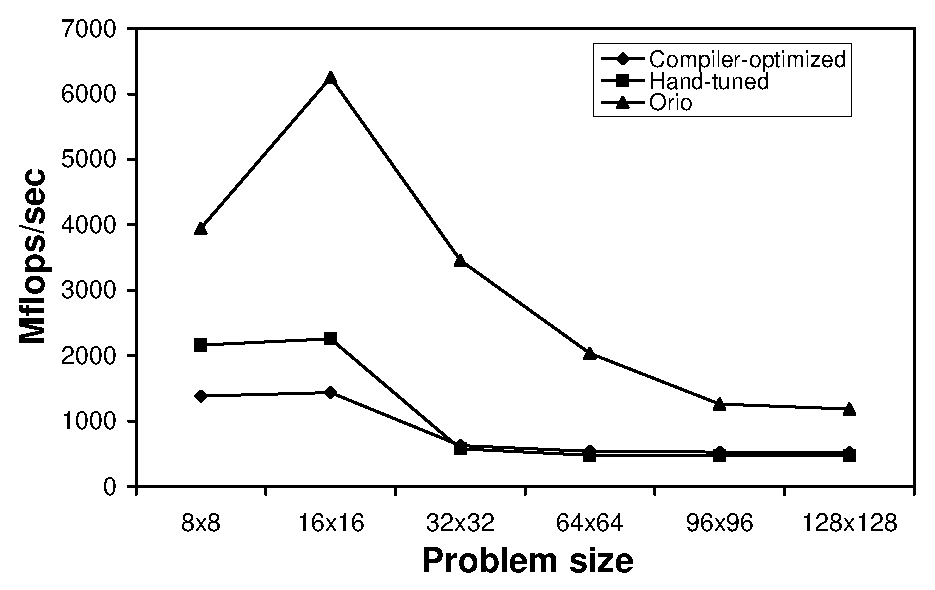
\includegraphics[width=.315\textwidth]{figures/ex27_cookie/smp.eps}
  \label{fig:ex27-cookie-smp} } \subfigure[Dual: $p=4$, $t/p=2$]{
  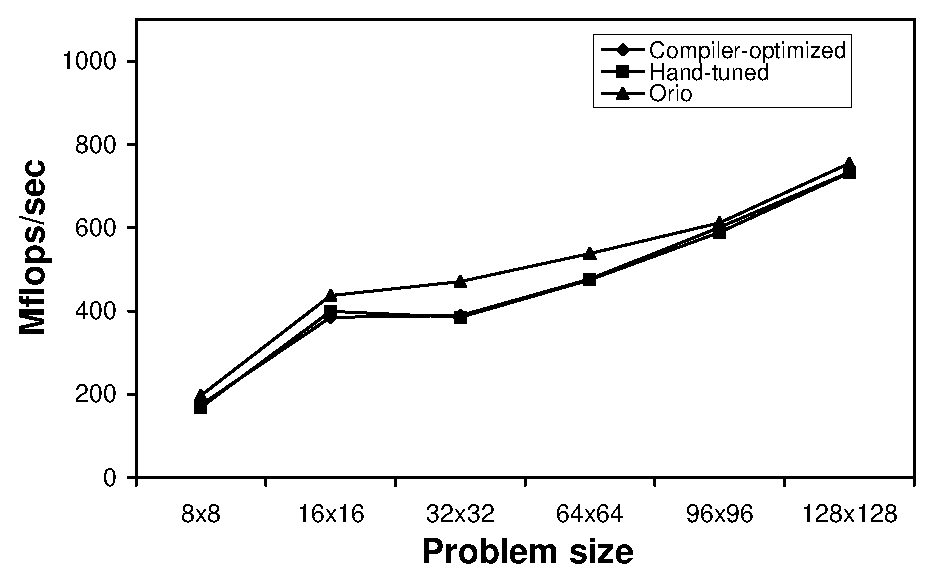
\includegraphics[width=.315\textwidth]{figures/ex27_cookie/dual.eps}
  \label{fig:ex27-cookie-dual} } \subfigure[VN: $p=8$, $t/p=1$]{
  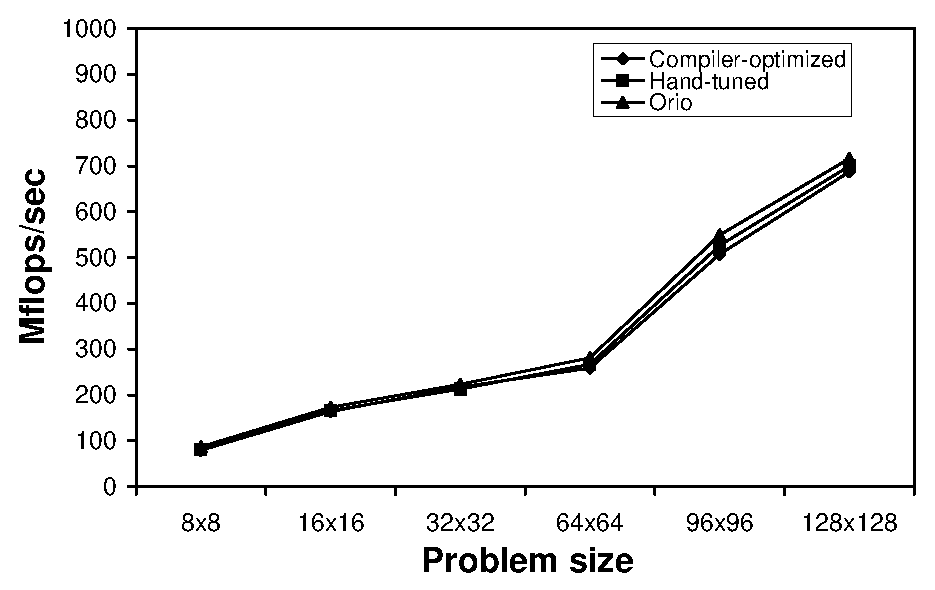
\includegraphics[width=.315\textwidth]{figures/ex27_cookie/vn.eps}
  \label{fig:ex27-cookie-vn} }
\end{center}
\caption{Performance of inode SpMV on eight-core Intel machine; $p$ is the number of processes, and $t/p$ is the threads per process.} 
\label{fig:ex27-cookie-results} 
\end{figure*} 

\begin{figure*} %[htb]
\begin{center} 
  \subfigure[1 node, SMP mode]{ 
  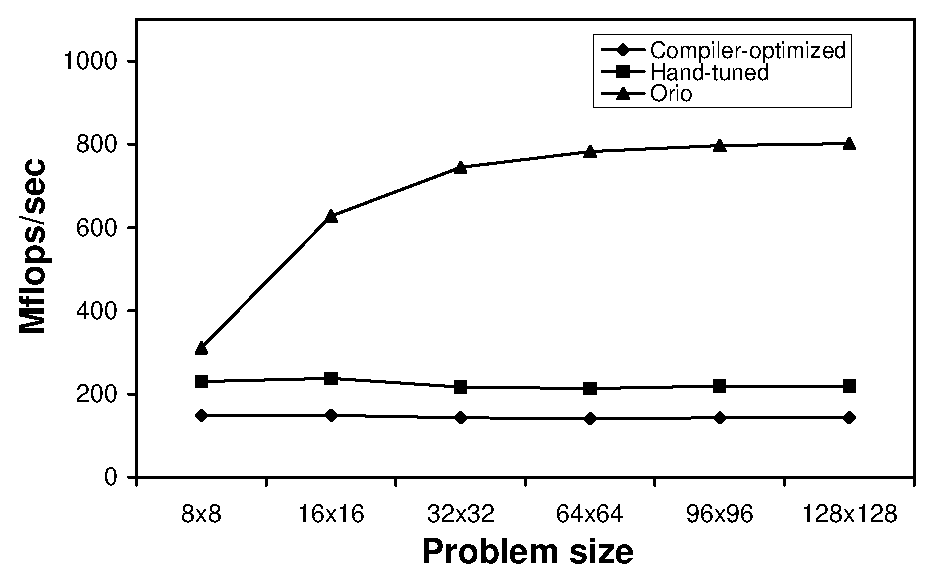
\includegraphics[width=.315\textwidth]{figures/ex27_bgp/n1_smp.eps}  
  \label{fig:ex27-bgp-smp-n1} 
  } 
  \subfigure[1 node, Dual mode]{ 
  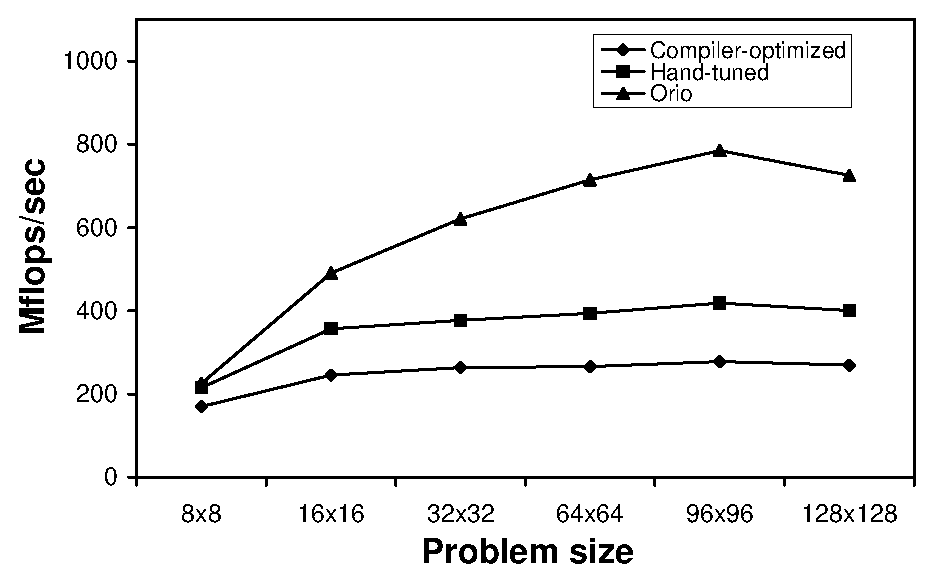
\includegraphics[width=.315\textwidth]{figures/ex27_bgp/n1_dual.eps}  
  \label{fig:ex27-bgp-dual-n1} 
  } 
  \subfigure[1 node, VN mode]{ 
  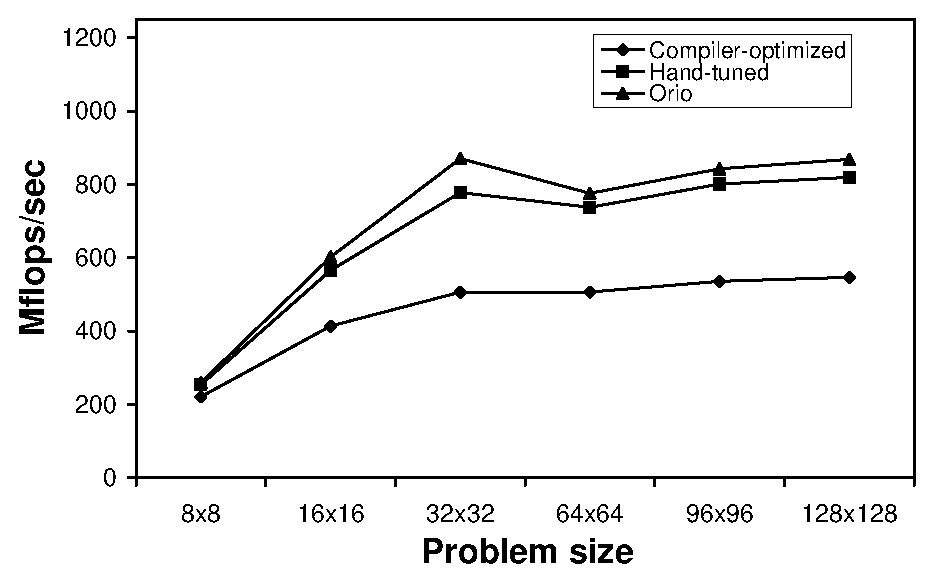
\includegraphics[width=.315\textwidth]{figures/ex27_bgp/n1_vn.eps}  
  \label{fig:ex27-bgp-vn-n1} 
  } 
  \subfigure[8 nodes, SMP mode]{ 
  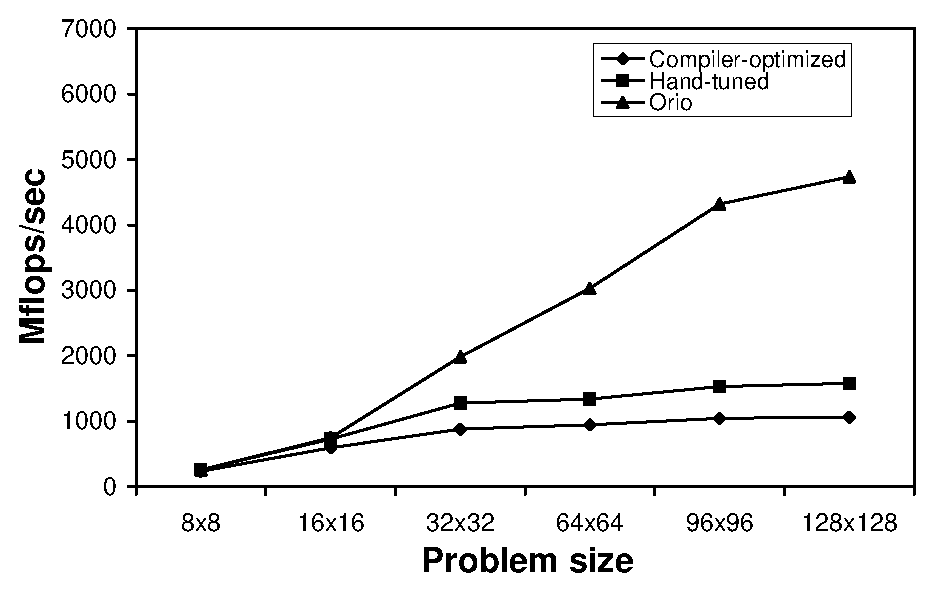
\includegraphics[width=.315\textwidth]{figures/ex27_bgp/n8_smp.eps}  
  \label{fig:ex27-bgp-smp-n8} 
  } 
  \subfigure[8 nodes, Dual mode]{ 
  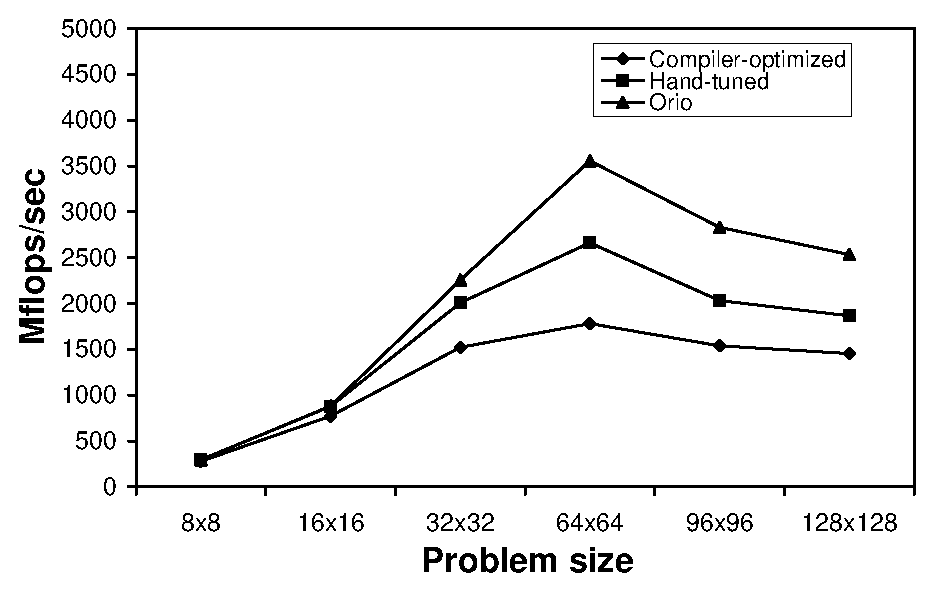
\includegraphics[width=.315\textwidth]{figures/ex27_bgp/n8_dual.eps}  
  \label{fig:ex27-bgp-dual-n8} 
  } 
  \subfigure[8 nodes, VN mode]{ 
  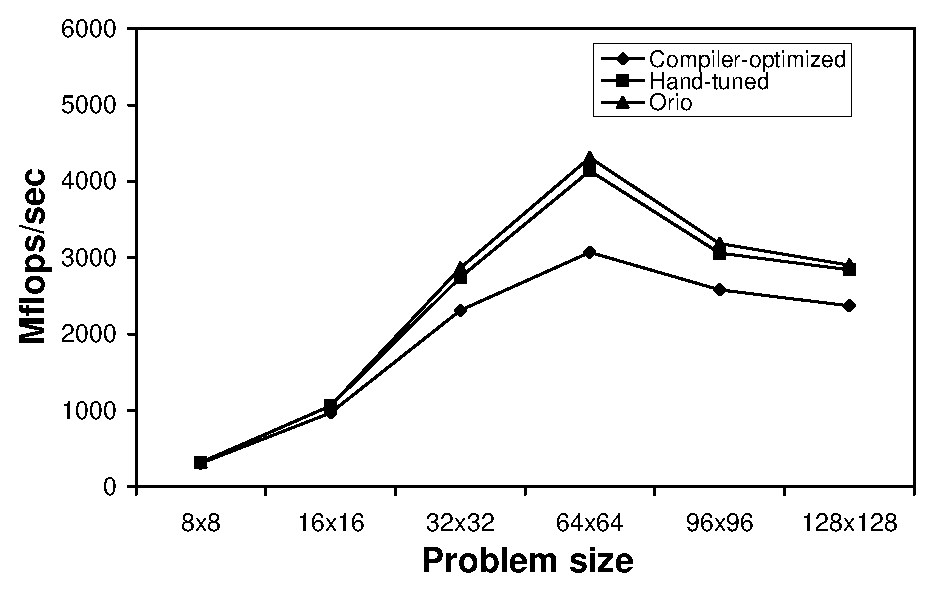
\includegraphics[width=.315\textwidth]{figures/ex27_bgp/n8_vn.eps}  
  \label{fig:ex27-bgp-vn-n8} 
  } 
%  \subfigure[32 nodes, SMP mode]{ 
%  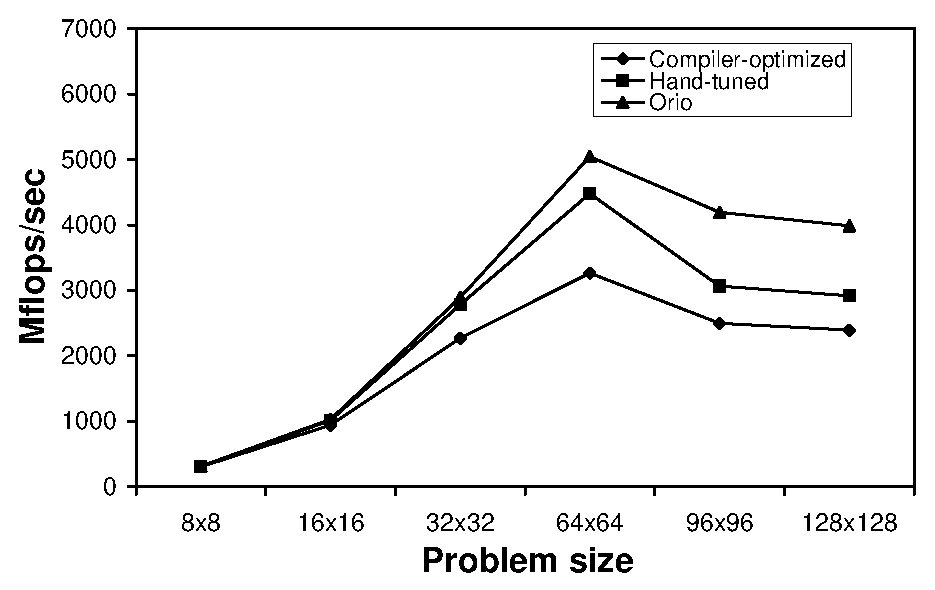
\includegraphics[width=.315\textwidth]{figures/ex27_bgp/n32_smp.eps}  
%  \label{fig:ex27-bgp-smp-n32} 
%  } 
%  \subfigure[32 nodes, Dual mode]{ 
%  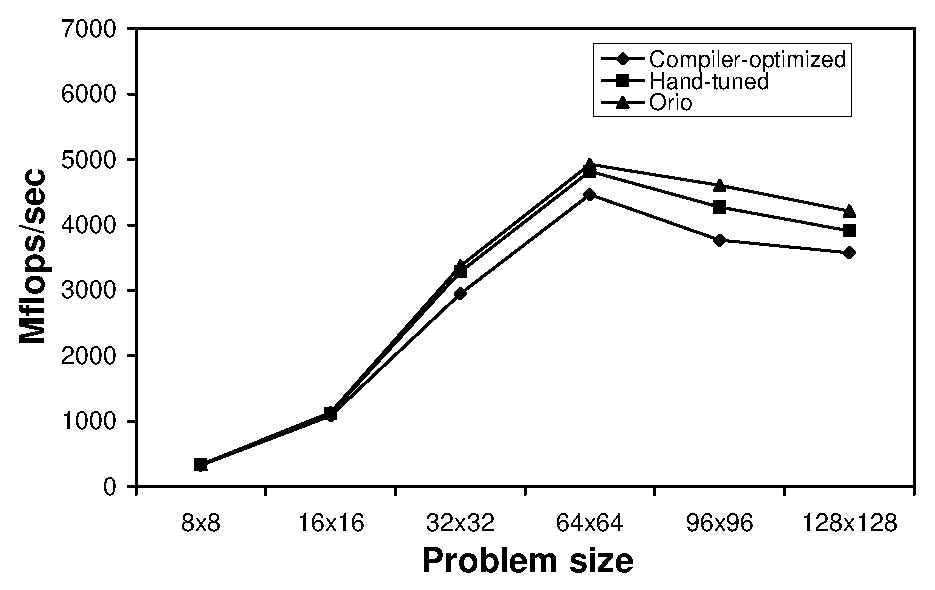
\includegraphics[width=.315\textwidth]{figures/ex27_bgp/n32_dual.eps}  
%  \label{fig:ex27-bgp-dual-n32} 
%  } 
%  \subfigure[32 nodes, VN mode]{ 
%  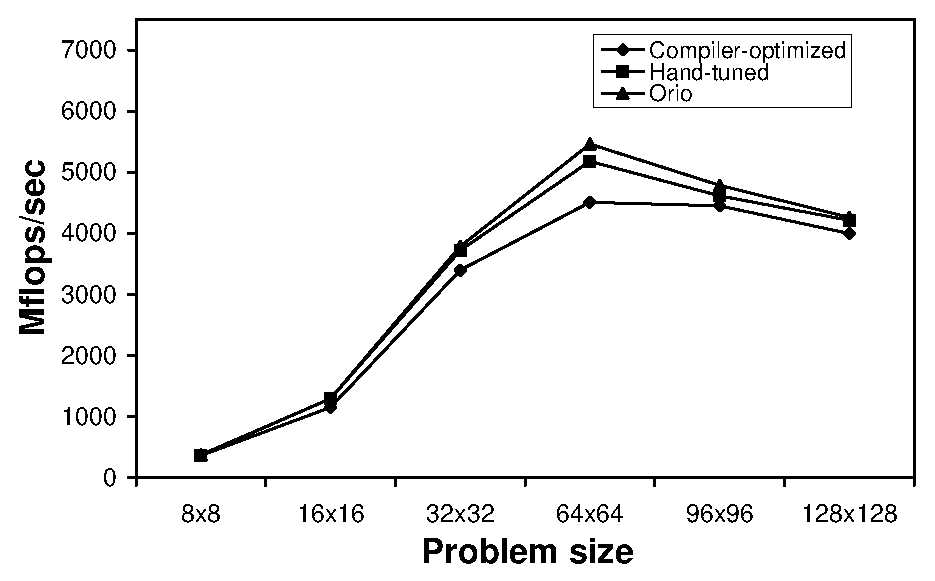
\includegraphics[width=.315\textwidth]{figures/ex27_bgp/n32_vn.eps}  
%  \label{fig:ex27-bgp-vn-n32} 
%  } 
\end{center}
\caption{Performance of inode SpMV on Blue Gene/P for 1 and 8 nodes.} 
\label{fig:ex27-bgp-results1} 
\end{figure*} 

\comment{
\begin{figure} 
\begin{center} 
  \subfigure[32x32, SMP mode]{ 
  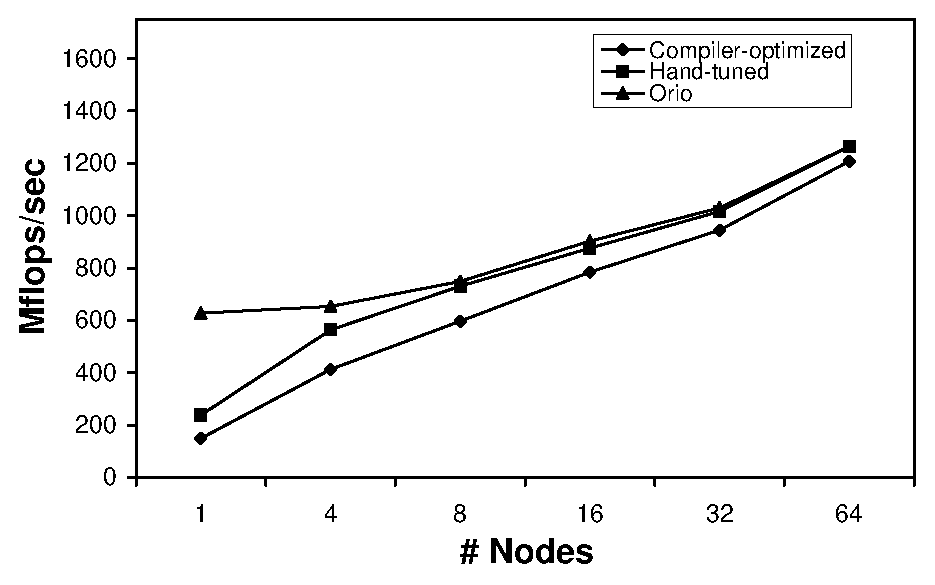
\includegraphics[width=.315\textwidth]{figures/ex27_bgp/s32_smp.eps}  
  \label{fig:ex27-bgp-smp-32x32} 
  } 
  \subfigure[32x32, Dual mode]{ 
  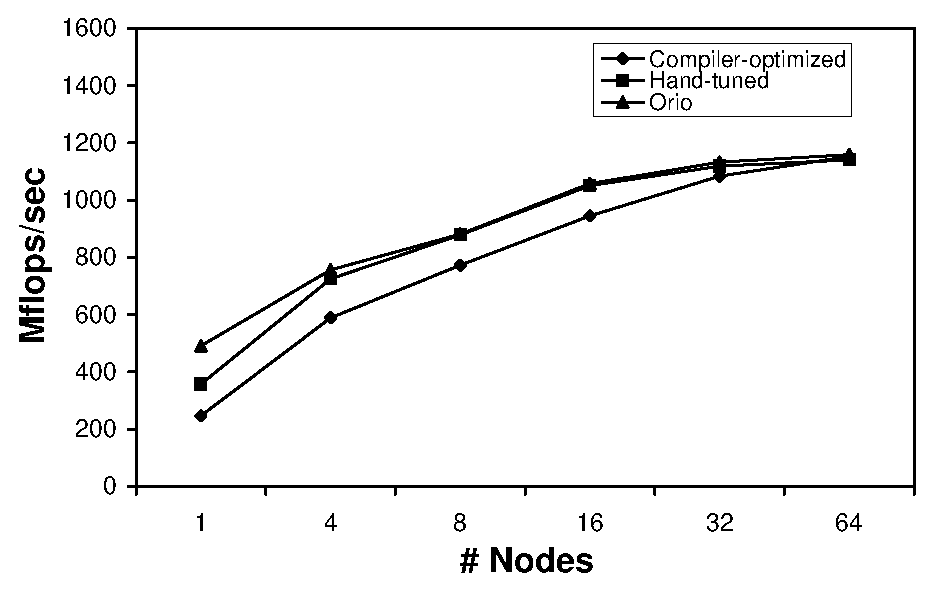
\includegraphics[width=.315\textwidth]{figures/ex27_bgp/s32_dual.eps}  
  \label{fig:ex27-bgp-dual-32x32} 
  } 
  \subfigure[32x32, VN mode]{ 
  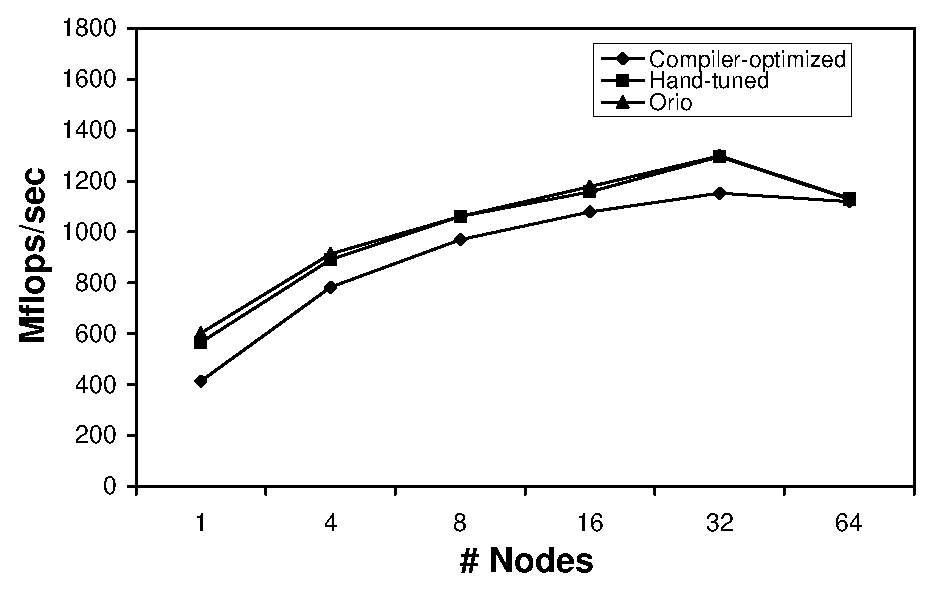
\includegraphics[width=.315\textwidth]{figures/ex27_bgp/s32_vn.eps}  
  \label{fig:ex27-bgp-vn-32x32} 
  } 
  \subfigure[64x64, SMP mode]{ 
  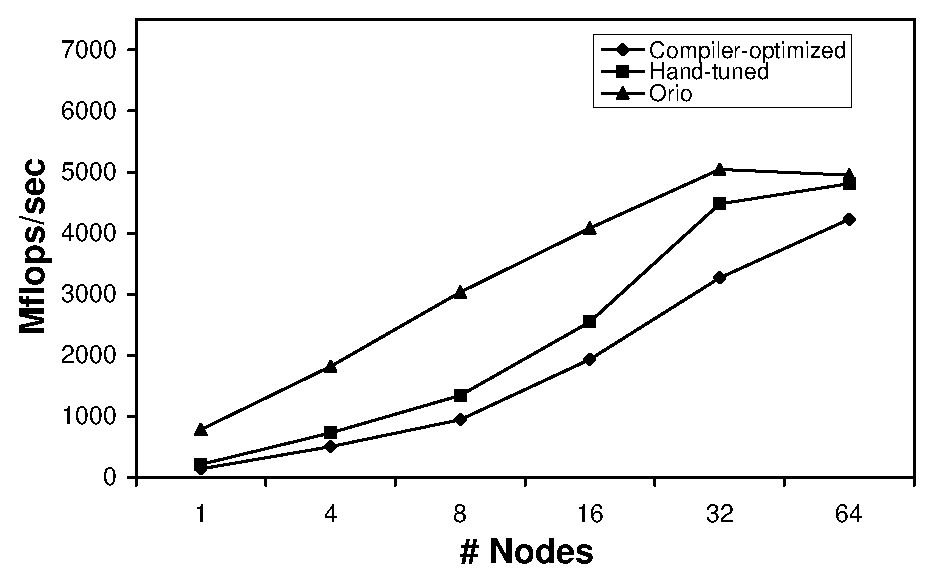
\includegraphics[width=.315\textwidth]{figures/ex27_bgp/s64_smp.eps}  
  \label{fig:ex27-bgp-smp-64x64} 
  } 
  \subfigure[64x64, Dual mode]{ 
  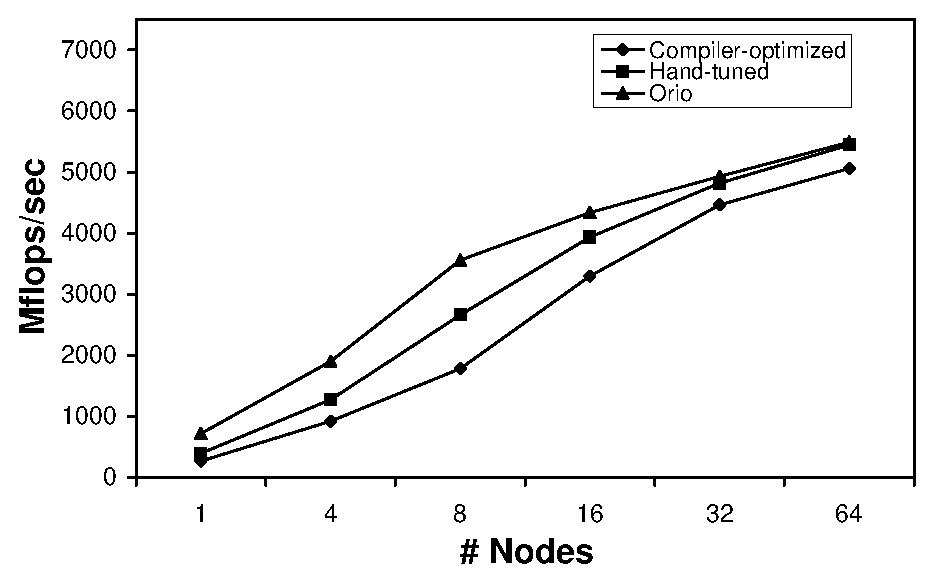
\includegraphics[width=.315\textwidth]{figures/ex27_bgp/s64_dual.eps}  
  \label{fig:ex27-bgp-dual-64x64} 
  } 
  \subfigure[64x64, VN mode]{ 
  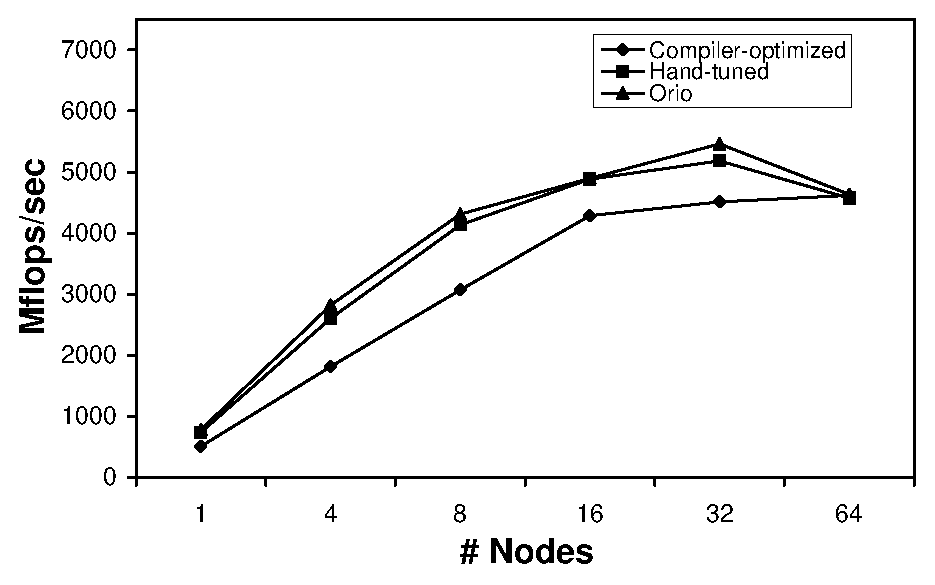
\includegraphics[width=.315\textwidth]{figures/ex27_bgp/s64_vn.eps}  
  \label{fig:ex27-bgp-vn-64x64} 
  } 
  \subfigure[128x128, SMP mode]{ 
  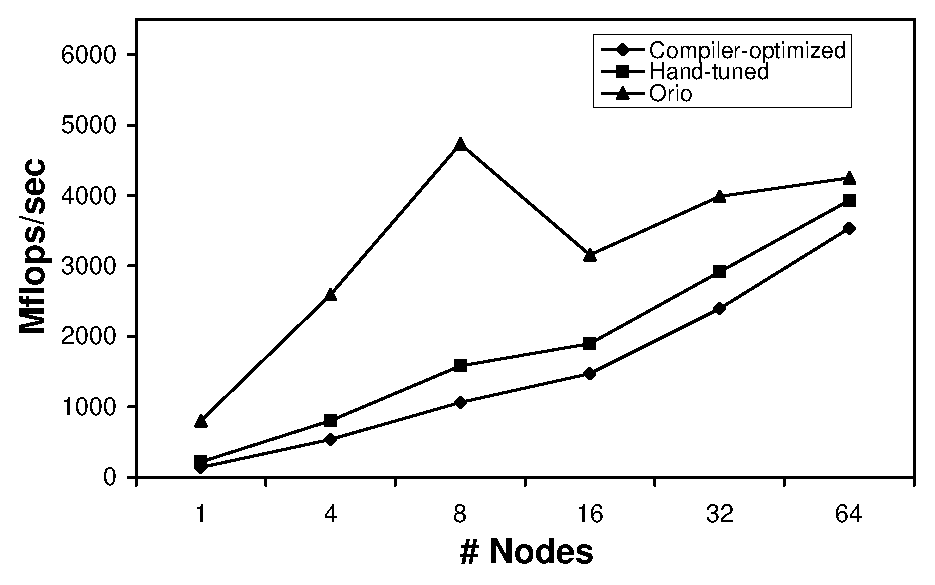
\includegraphics[width=.315\textwidth]{figures/ex27_bgp/s128_smp.eps}  
  \label{fig:ex27-bgp-smp-128x128} 
  } 
  \subfigure[128x128, Dual mode]{ 
  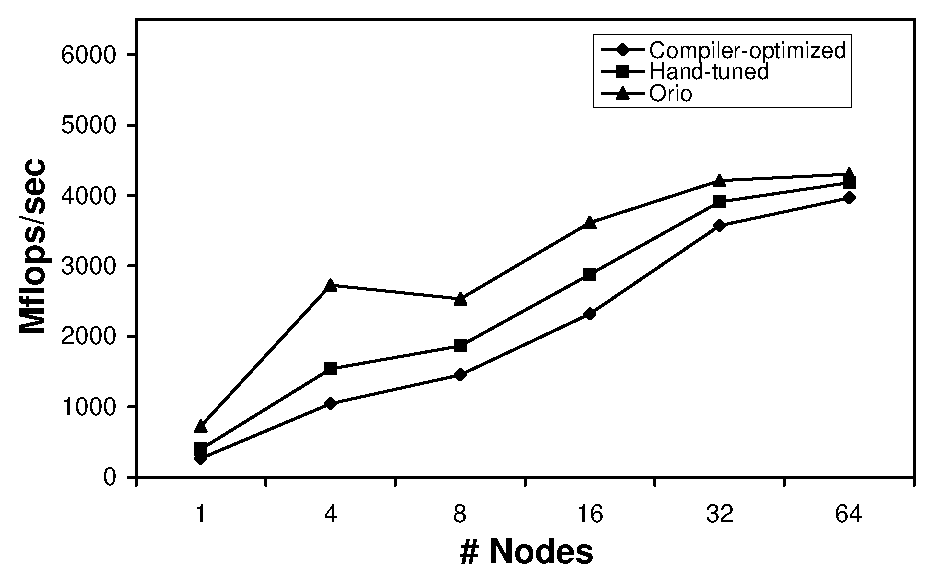
\includegraphics[width=.315\textwidth]{figures/ex27_bgp/s128_dual.eps}  
  \label{fig:ex27-bgp-dual-128x128} 
  } 
  \subfigure[128x128, VN mode]{ 
  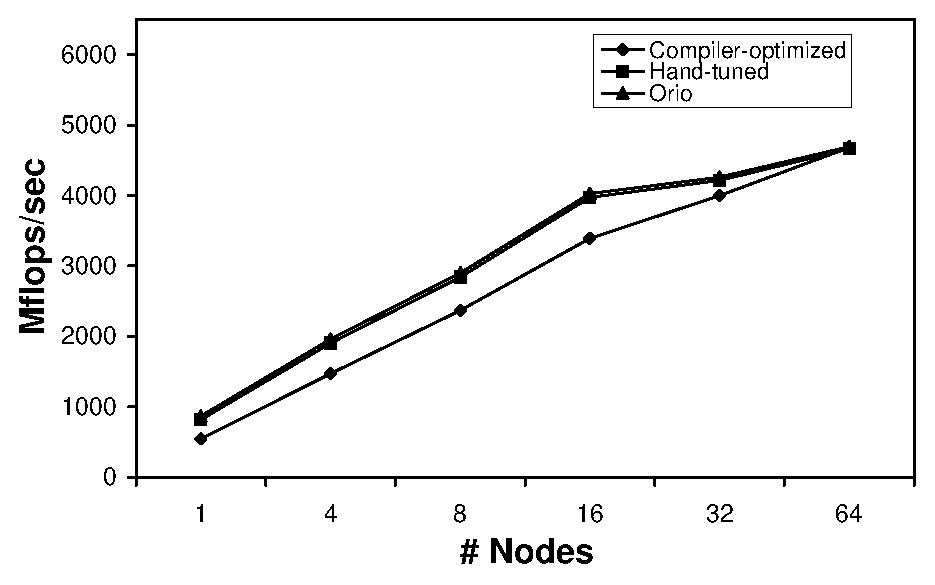
\includegraphics[width=.315\textwidth]{figures/ex27_bgp/s128_vn.eps}  
  \label{fig:ex27-bgp-vn-128x128} 
  } 
\end{center}
\caption{Performance of inode SpMV on Blue Gene/P for problem sizes 32x32, 64x64, and 128x128.} 
\label{fig:ex27-bgp-results2} 
\end{figure} 
}



Figure~\ref{fig:ex27-cookie-results} shows the performance results on the
Intel Xeon. The problem size is the number of grid points in the $x$ and $y$
directions, not the size of the sparse input matrix. The matrix dimension is
based on the grid size and the number of field components computed for each grid
point; for example, an $8 \times 8$ problem involves sparse matrices of
dimension 900 with 17,040 nonzero entries. In this experiment, we ran in
three multicore modes: SMP (one MPI process, eight
threads/process), dual (four MPI processes, two threads/process), and virtual
node or VN (eight MPI processes, one thread/process). The code tuned by Orio
consistently outperforms the others. Furthermore, the performance of
the hand-tuned code is almost equivalent to that of the icc-optimized simple
code. Performance differences between the Orio version and the hand-tuned
version become more significant as more threads per process are employed to
facilitate OpenMP parallelization. The SMP and VN results show that
optimizations using loop-level parallelism (through OpenMP) achieve much
better performance than using MPI coarse-grained parallelism.
%Moreover, for the multithread cases, tuning using Orio determined that
%the performance benefit of SIMDization is more significant than that of
%thread-level parallelization only when the problem sizes are small. The
%reason for this is due to the overhead introduced by OpenMP from coordinating
%its threads across processors.
%So, each optimized
%code for the many-thread cases comprises two distinct tuned codes to handle

The Blue Gene/P results in Figure~\ref{fig:ex27-bgp-results1} again show
%Blue Gene/P was done for a varied number of nodes (i.e., 1, 8, and 32)
%and the same three different parallel modes as before (i.e., SMP,
%dual, and VN). 
that empirical optimization using Orio produces the best performance for
all cases. 
%outperforming both the hand-tuned and the xlc-optimized codes. 
On this architecture, the performance gap between the xlc-optimized and the
hand-tuned codes is now larger than in the Intel experiment. Similarly, by
exploiting thread-level parallelism, the Orio-optimized code performs better
than the hand-tuned version when the number of threads per process increases
and the number of nodes decreases. For the single-thread cases (VN mode),
thread-level parallelism is not exploited; nevertheless, the Orio version
still performs better than the other two choices.
%This validates the
%effectiveness of Orio in empirically tuning sequential codes.

\subsection{Evaluation of the Pluto-Orio Integrated System} 

This section discusses the performance evaluation of the integrated
Pluto-Orio system (discussed in Section~\ref{sec:integration}) on the
multicore Intel Xeon by using a number of application kernels that are
nontrivial to optimize and parallelize. We compare the performance of the
code tuned by Orio with the base code and the Pluto-generated codes. The
Pluto code was obtained by running the base code with
Pluto-0.3.0~\cite{pluto030} using \texttt{--tile} to employ loop tiling for
L1 cache, \texttt{--l2tile} to employ loop tiling for L2 cache, and
\texttt{--unroll} to employ loop unrolling, and for parallel code generation,
an additional \texttt{--parallel} option. We used Pluto's default tile
sizes (L1: 32x32 or 32x32x32; L2: 256x256 or 256x256x256) and default
unroll factors (64 for 1-D unrolling and 8x8 for 2-D
unroll/jamming). All codes were compiled with the Intel C compiler
using the \texttt{-O3} optimization flag to enable auto-vectorization
and other advanced optimizations, and
\texttt{-parallel} (or \texttt{-openmp} in the case of manual OpenMP parallelization) 
to enable code parallelization.
 
In the following sections, we refer to the icc-optimized base code as
xs``ICC,'' the Pluto-generated code with L1 tiling and
unroll/jamming as ``Pluto (L1 tiling),'' and the Pluto-generated code with L1
and L2 tilings and unroll/jamming as ``Pluto (L1+L2 tiling).'' The code
tuned by Orio is referred to as ``Pluto+Orio.''

\begin{figure*}%[htb] 
\begin{center} 
  \subfigure[Sequential (T=500)]{ 
  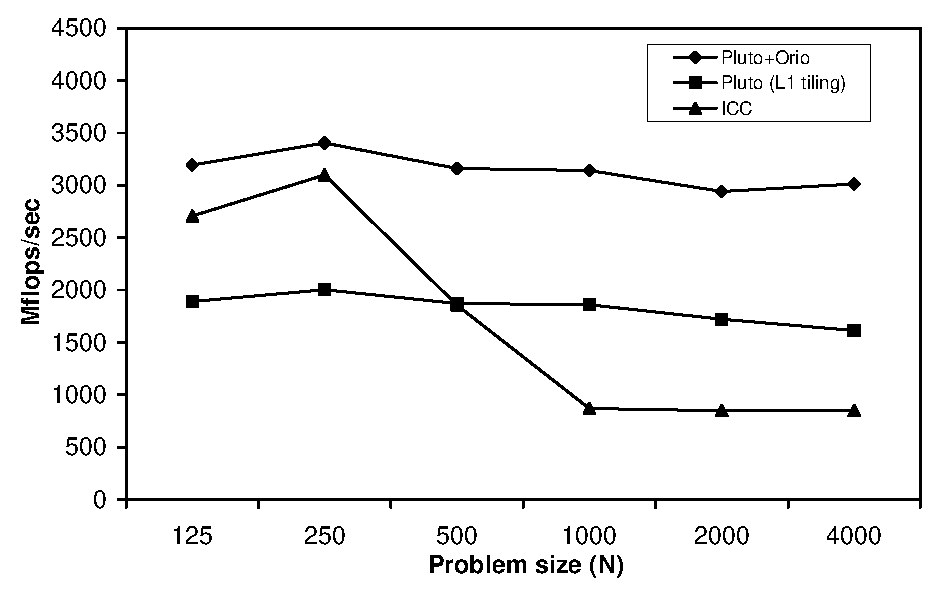
\includegraphics[width=.45\textwidth]{figures/fdtd-2d-cookie/seq.eps} 
  \label{fig:fdtd-2d-cookie-seq} } \subfigure[Parallel (T=500, 
  N=2000)]{ 
  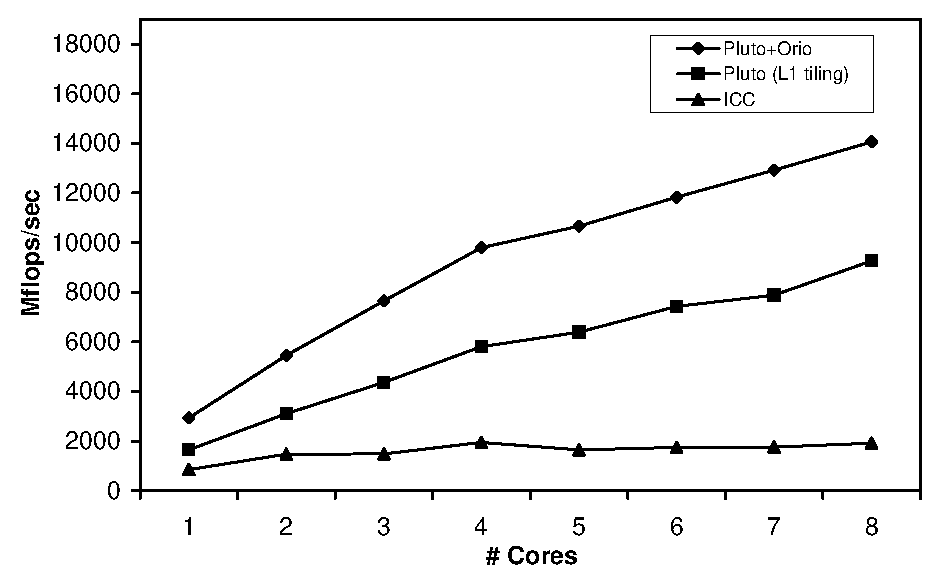
\includegraphics[width=.45\textwidth]{figures/fdtd-2d-cookie/par.eps} 
  \label{fig:fdtd-2d-cookie-par} } 
\end{center}
\caption{2-D FDTD performance on an eight-core Intel Xeon.} 
\label{fig:fdtd-2d-cookie-results} 
\end{figure*} 

\begin{figure*}%[htb]
\begin{center} 
  \subfigure[Sequential (T=500)]{ 
  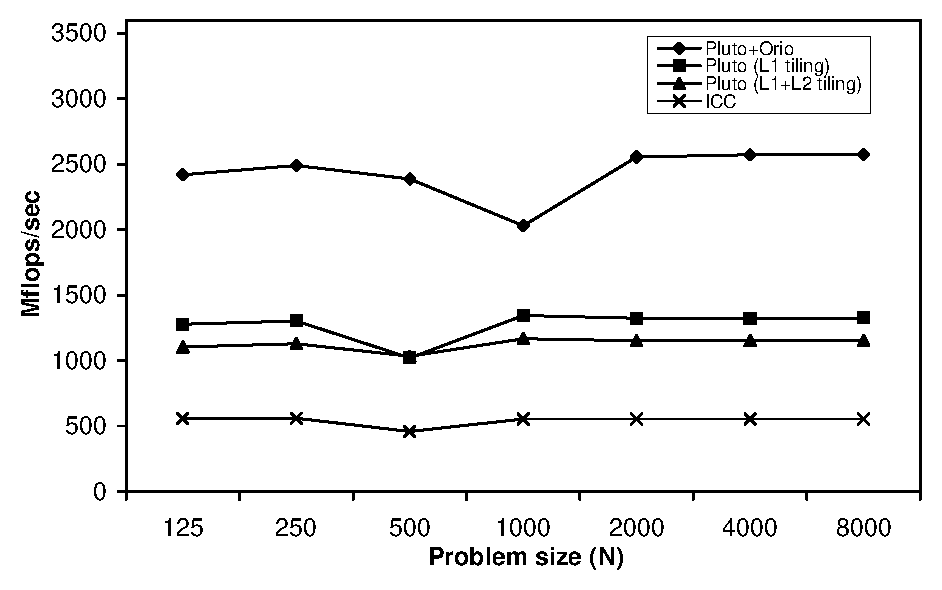
\includegraphics[width=.45\textwidth]{figures/seidel-cookie/seq.eps} 
  \label{fig:seidel-cookie-seq} } \subfigure[Parallel (T=500, 
  N=4000)]{ 
  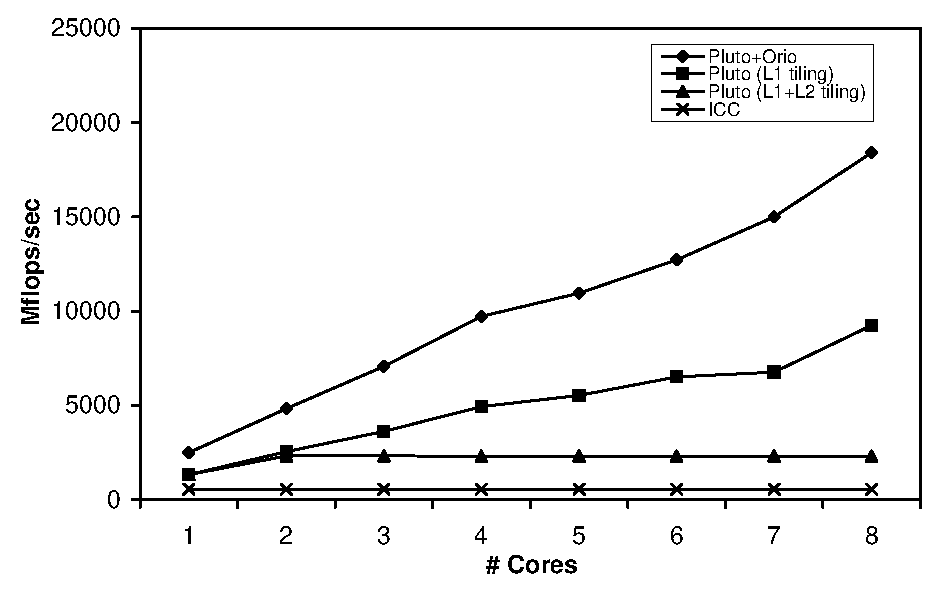
\includegraphics[width=.45\textwidth]{figures/seidel-cookie/par.eps} 
  \label{fig:seidel-cookie-par} } 
\end{center}
\caption{3-D Gauss-Seidel performance on eight-core Intel machine.} 
\label{fig:seidel-cookie-results} 
\end{figure*} 

\begin{figure*}%[htb]
\begin{center} 
  \subfigure[Sequential]{ 
  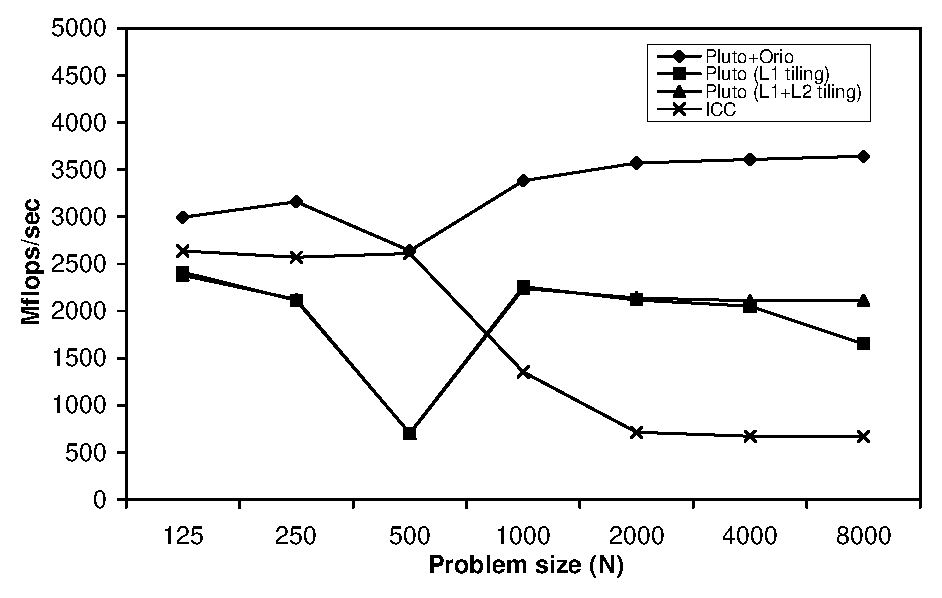
\includegraphics[width=.45\textwidth]{figures/lu-cookie/seq.eps} 
  \label{fig:lu-cookie-seq} } \subfigure[Parallel (N=4000)]{ 
  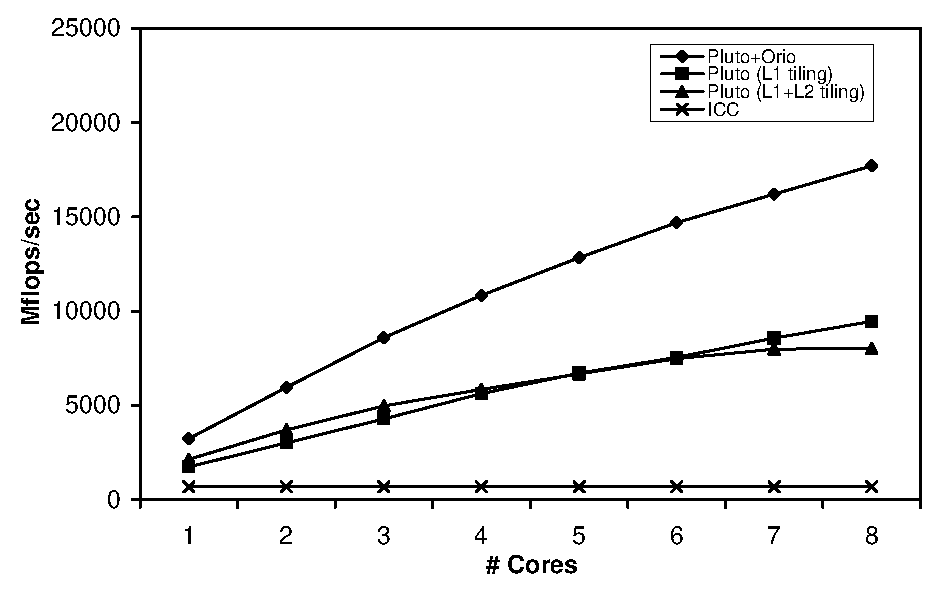
\includegraphics[width=.45\textwidth]{figures/lu-cookie/par.eps} 
  \label{fig:lu-cookie-par} } 
\end{center} 
\caption{LU Decomposition performance on eight-core Intel machine.} 
\label{fig:lu-cookie-results} 
\end{figure*} 


 
\subsubsection{2-D Finite-Difference Time-Domain Method for Computational Electromagnetics}  
We consider the two-dimensional finite difference time domain (FDTD)
algorithm, a popular method for solving the time-dependent Maxwell's
equations in the context of computational electrodynamic problems. As
shown in Figure~\ref{fig:fdtd-2d-code}, the 2-D FDTD method is
implemented as an outer iteration over time containing four
imperfectly nested loops.  The arrays $ex$ and $ey$ denote the
electric field components, and the array $hz$ denotes the magnetic
field.


\begin{figure}
\begin{center}
\begin{minipage}{3in} 
\scriptsize
\begin{verbatim} 
for(t=0; t<tmax; t++) { 
  for (j=0; j<ny; j++) ey[0][j] = t; 
  for (i=1; i<nx; i++) 
    for (j=0; j<ny; j++) 
      ey[i][j] -= 0.5*(hz[i][j] - hz[i-1][j]); 
  for (i=0; i<nx; i++) 
    for (j=1; j<ny; j++) 
      ex[i][j] -= 0.5*(hz[i][j] - hz[i][j-1]); 
  for (i=0; i<nx; i++) 
    for (j=0; j<ny; j++) 
      hz[i][j] -= 0.7*(ex[i][j+1] - ex[i][j]
                  + ey[i+1][j] - ey[i][j]); 
} 
\end{verbatim} 
\end{minipage} 
\end{center}
\caption{2-D FDTD code.} 
\label{fig:fdtd-2d-code} 
\end{figure}

\begin{figure}%[ht]
\begin{center}
\begin{minipage}{3in} 
\scriptsize
\begin{verbatim} 
for (t=0; t<=T-1; t++) 
  for (i=1; i<=N-2; i++) 
    for (j=1; j<=N-2; j++) 
      A[i][j] = (A[i-1][j-1] + A[i-1][j] 
          + A[i-1][j+1] + A[i][j-1] + A[i][j] 
          + A[i][j+1] + A[i+1][j-1] + A[i+1][j] 
          + A[i+1][j+1]) / 9.0; 
\end{verbatim} 
\end{minipage} 
\end{center}
\caption{3-D Gauss-Seidel code} 
\label{fig:seidel-code} 
\end{figure}

\begin{figure}%[ht]
\begin{center}
\begin{minipage}{2.8in} 
\scriptsize
\begin{verbatim} 
for (k=0; k<=N-1; k++) { 
  for (j=k+1; j<=N-1; j++) 
    A[k][j] /= A[k][k]; 
  for(i=k+1; i<=N-1; i++) 
    for (j=k+1; j<=N-1; j++) 
      A[i][j] -= A[i][k]*A[k][j]; 
} 
\end{verbatim} 
\end{minipage} 
\end{center}
\caption{LU decomposition code.} 
\label{fig:lu-code} 
\end{figure}


The performance of the sequential 2-D FDTD code for $tmax=500$ and $nx=ny$ is
shown in Figure~\ref{fig:fdtd-2d-cookie-seq}. The base code optimized by icc
alone performs better than Pluto for small problem sizes since all input
arrays fit in the L2 cache (insufficient computation to offset Pluto's tiling
overhead). As the array sizes increase, the lack of data reuse impairs the
base code's performance, whereas the Pluto performance remains about the
same.
%We used Orio to generate two code variants: one for small problem sizes
%and another for large problem sizes. 
When the input arrays are small, Orio discovers that applying
Pluto's polyhedral transformations is not beneficial, and therefore
it employs only its syntactic transformations on the original FDTD
code. For large problem sizes, Orio exploits some of the Pluto's code
transformations and enhances these further with its syntactic
optimizations, resulting in performance consistently and significantly
higher than both the base and Pluto codes (up to 86\% over Pluto).


%By tuning the sequential code with Orio,
%the attainable performance enhancement over Pluto is up to 86\%.
 
Figure~\ref{fig:fdtd-2d-cookie-par} shows the multicore performance
obtained for $tmax=500$ and $nx=ny=2000$. The results indicate that
whereas icc is unable to autoparallelize the code, Pluto detects the
existence of pipelined parallelism and then successfully parallelizes
the code. Locality-exploiting optimizations by Orio additionally
improve the Pluto performance by up to 78\%. Moreover, we observe
that because of memory contention between the two quad-core Intel
processors, the speedup of both the Pluto and Orio codes slightly
decreases when the number of cores used is greater than four.
 
%%BN: commented out since this needs more explanation (no room in this version)
%It is to be noted that collecting performance results of the Pluto 
%code with L1 and L2 tilings was not possible because of the large code 
%size of the generated loop nest, which led to an impractically huge 
%compile time. 

\subsubsection{3-D Gauss-Seidel Successive Overrelaxation Method}  
Figure~\ref{fig:seidel-code} shows the 3-D Gauss-Seidel computation, 
which is sometimes referred to as
\emph{successive displacement method}, indicating the dependence of the 
iterations on the ordering. If the ordering is changed, the components
of the new iterations will change as well.

Figure~\ref{fig:seidel-cookie-seq} contains the sequential performance
results for $T=500$, which show that applying Pluto's polyhedral tiling on
the original code always delivers performance boosts, which range from 126\%
to 142\%. When using Pluto, performing two-level tiling (for both L1 and L2
caches) yields 13\% lower performance than performing only L1 tiling. 
This is also reflected in the best sequential code found by Orio, where
one-level tiling (for L1 cache only) is always performed. The sequential
speedup obtained from tuning the Pluto code with Orio is significant, ranging
from 51\% to 133\%.

The parallel performance results for $T=500$ and $N=4000$ are shown in
Figure~\ref{fig:seidel-cookie-par}. Again we observe that icc failed to
parallelize the code, whereas Pluto was able to parallelize it and Orio
improved the performance of the one-level tiled Pluto code further by up to
128\% (and up to 548\% for the two-level tiled Pluto code). We observed that
tiling over both L1 and L2 can result in worse performance than L1-only
tiling because the number of tiles can be smaller than the number of cores.
%Similar earlier trend also exists
%in these performance results: Pluto parallelizes the code through its
%polyhedral transformations (i.e., skewing and tiling), while the icc
%compiler alone does not parallelize the loop. Empirical tuning via
%Orio creates up to 122\% speedups over the one-level tiled Pluto code,
%and up to 548\% speedups over the two-level tiled Pluto code. Another
%finding is that tiling for both L1 and L2 caches contributes to a poor
%scalability because the number of tiles can be less than the number of
%processors, resulting in underutilization of the available resources.


\subsubsection{LU Factorization}  
 
LU factorization or decomposition is a numerical method for the
solution of linear systems of equations; a simple implementation is
shown in Figure~\ref{fig:lu-code}.


The sequential performance results are shown in
Figure~\ref{fig:lu-cookie-seq}. Similarly to the 2-D FDTD results, the icc-optimized code is more
efficient than the Pluto-generated codes when the input arrays are small and
fit in the L2 cache. Because of better data locality, however, the
performance of the Pluto-tiled codes is better than that of the base code as
the input arrays get larger. 
%Again, there are two different codes generated
%by Orio: one for small problem sizes and one for large problem sizes. And
Consequently, Orio employs Pluto's polyhedral transformations only for large
input sizes prior to applying its own syntactic transformations. 
%Unlike 3-D
%Gauss-Seidel, this time Orio chooses to apply both L1 and L2 tilings when
%generating the best tuned code. 
Compared to the two Pluto codes, the
Orio-tuned code yields performance improvements ranging between 26\% and 277\%.

The parallel performance results shown in Figure~\ref{fig:lu-cookie-par} were
obtained for $N=4000$. We observe that icc is not able to parallelize the
code, whereas Pluto achieves higher performance by exploiting multicore
parallelism. Furthermore, both Pluto-generated codes have comparable
performance, with slightly better scalability exhibited by the single-level tiled
code. Orio further improved the performance of the Pluto-generated versions
by a factor of 51\% to 120\%.
 
